\documentclass[a4paper,fontsize=12pt]{article}
\usepackage{fontspec}                 % loaded by polyglossia, but included here for transparency
\usepackage{polyglossia}
\usepackage{indentfirst}              % Insert "Red line"

\setmainlanguage{russian}
\setotherlanguage{english}

\usepackage{graphicx}         % Insert images
\usepackage{siunitx}          % for \ang macros
\usepackage{units}            % for fraction with unit

\sisetup{
   list-final-separator = {\ и \ },
   range-phrase = {\ до\ }
  }

\DeclareSIUnit\siion{ион}

\usepackage[left=3.5cm,right=2cm,top=2.5cm,bottom=2.5cm,bindingoffset=0cm]{geometry}
% XeLaTeX can use any font installed in your system fonts folder
% Linux Libertine in the next line can be replaced with any
% OpenType or TrueType font that supports the Cyrillic script.

\newfontfamily\russianfont[Script=Cyrillic]{Arial}

\newcommand{\kev}{кэ\uppercase{В}}

\begin{document}

% \maketitle\clearpage
% \restoregeometry
% \pagenumbering{arabic}
% \tableofcontents\clearpage

%

\begin{titlepage}
  \thispagestyle{empty}

  \begin{center}
    \Large{\textbf{Национальный исследовательский университет МИЭТ}}

    \vspace{5cm}

    \huge{\textbf{\textit{Курсовая работа}}}

    \large{по дисциплине}

    \large{«Квантовая теория и статистическая физика»}

    \vspace{5cm}

    % \huge{\textbf{\textit{Оценка апроксимации для эффективной топографической симуляции ионно-лучевых процессов: 10К эВ $Ar$ на $Si$}}}
  \end{center}

  \vspace{1cm}

  \begin{flushright}
    \textbf{Выполнил:}                  \linebreak
    Студент группы ЭКТ-26               \linebreak
    Чечетин П. Е.                       \linebreak
    \textbf{Проверил:}                  \linebreak
    % учёная степень, учёное звание       \linebreak
    Румянцев Александр                   \linebreak
  \end{flushright}

  \vfill

  \begin{center}
    \Large{Москва – 2013}
  \end{center}
\end{titlepage}

\newpage

\tableofcontents

\newpage
\part{Оценка апроксимации для эффективной топографической симуляции ионно-лучевых процессов: 10 \kev{} $Ar$ на $Si$}
\section{Резюме}
Основное предположение о существовании эффективной топографической симулиции состоит в том что распыление - это локальный процесс который зависит только от угла столкновения и не зависит от формы поверхности. Если учитывать переосаждение, распылённые атомы переосаждаются и не вызывают дальнейшего распыления когда они сталкиваются с другим участками поверхности. Более того угловое распределение распылённых атомов определяется законом косинуса. Если учитывать ионное отражение, тогда ионы не теряют энергию в процессе обратного рассеяния. Используя симуляцию бинарных столкновений ($IMSIL$) и сравнивая их с результатами полученными с помощью топографического симулятора ($IonShaper^{®}$) мы видим что всем этим предположениям нужны уточнения для симуляции наноструктур прнебрегая распыление распылённых атомов. Кроме того мы показываем что не локальные модели в основном справедливы для ионно-лучевого наведённого облучения внутренней структуры.


\section{Введение}
Ионные лучи это многостароннее и всё больше используемое стредства для создания наноструктур либо c помощью прямого фрезерования либо путём процессов в газовой среде. Настоящее обучение мотивированно усилиями создать штампы для нано-литографии c массивными многоионными лазерными системами. Во всех приложениях симуляция может помочь понять физические процессы и оптимизировать форму структур.


\begin{figure}[h]
    \centering
    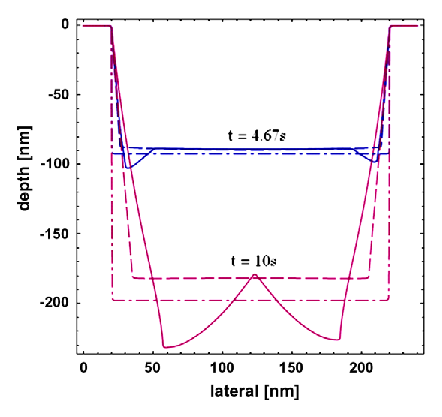
\includegraphics[width=6cm]{images/part1/1.eps}
    % Trenches sputtered by a 200 nm wide 10 keV Ar beam with a current density of 10 mA/cm2 after 4.67 and 10 s.
    \caption{Яма рысплённая лучём 10 \kev{} 200 нм шириной c плотностю тока \SI[per-mode=fraction]{10}{\kilo\g\milli\ampere\per\square\centi\meter} }
    \label{fig:part1TrenchShape}
\end{figure}

Большинство сущестувующих алгоритмов для численно эффективных топографических симуляции ионно-лазерных процессов моделирует поверхность проникновения явно, в соответствии с историей, точки поверхности считались соединёнными прямыми сегментами. Все алгоритмы базируются на предположении что рассеивание - это функция угла между направлением ионов и локальной нормалью поверхности. Обычно это хорошая апрокимация для структур в диапозоне микрометров, но это становится под вопросом когда характерный размер становится меньше. Только некоторые алгоритмы включают переосаждение и только несколько распыление отраженных ионов. Эти эффекты в основном важны в структурах с большим отношением сторон как в глубоких ямах. Рис. ~\ref{fig:part1TrenchShape} показывает контуры ям облучённых 200 нм широко гомогенным ионным лучём в два раличных момента времени, посчитанных с помощью програмного обеспечения $IonShaper^{®}$. В любое время симуляция без переосаждения и отражения (штрих-пунктирная линии) сравнима с симуляцией учитывающей только переосаждение (пунктирная линия) и учитывающей как переосаждение так и отражение (сплошная линия). Можно заметить что переосаждение атомов рассееных из дна ямы ведёт к уменьшению ямы по направлению ко дну. На следующей стадии (не показанно), переосаждение от граней ко дну и к другой грани ведёт к уменьшению эфективности фрезерования. Отражение ионов от граней ведёт к формированию микроям на дне ямы возле граней. Более того, увеличение излучение на наклонёную поверхность микротрещин ведёт к дополнительному переосаждению на грани.

В подсчёте переосаждённого потока, закон косинуса используется чтобы описать угловое распределение распылённых ионов. Обратное рассеение предпологаеться без потери энергии. Далее, распылённые атомы которые достигают другую точку поверхности переосаждаясь там и не вызывают рассеение. Эти предположения как и локальная аппрокимация рассеения исследуются в этой статье используя симуляцию бинарных столкновений. Мы ограничиваем себя в 10 \kev{} $Ar$-ионы и $Si$-мишени т.к. это наш текуший фокус интересов.

\section{Симуляция}
\subsection{Топографическая симуляция}

Двухмерная(2D) топограческая симуляция выполняются с $IonShaper^{®}$ программой. Коротко, поверхность описывается достаточным кол-вом точек которые движутся перпендикулярно к среднему наклону смежных сегментов. Скорость точек считается от потока атомов распылённых ионным лучом и от ионов отражённых от других частей поверхности и от потока переосаждённых атомовов исходящих от распыления от остальных точек поверхности. Распыление считается локальным процессом, т.е. поток распылённых частиц в определённой точке пространства зависит только от потока падаюших ионов в эту точку и их угла относительной нормальни поверхности.

В действительности, из-за ограниченных пределов отскока, распылённые атомы испускаются из облости вокруг точки падения. Чтобы исследовать этот эффект мы дополнительно реализовали не локальную модель потока расплыления. Кол-во отскоков в определённой точке поверхности (точке назначения) от столкновения ионов в другой точке поверхности (источнике) расчитывается от расстояния между двух точек и угла между прямой соединяющей эти точки и направлением падающих ионов.

Изначальная версия $IonShaper^{®}$ включала модель вынужденного лучевого напыления которое включало посчёт предшествующей зоны наблюдения и простую реализацию нелокального эффекта ионов/напылении. Было показанно что доля напыления пропоруианальна кол-ву отскоков достигших поверхность. Поэтому мы улучшили модель напыления используя модель основанную на отскоках опиисанную выше.

\subsection{Бинарная симуляция столкновений}

Бинарная симуляция столкновений сделанна с IMSIL алгоритмом. IMSIL было использованно для имплантационных исследований для одна и двух мерных целей. В этой работе мы только используем аморфные цели, т.к. $Si$ просто аморфиризуется при ионом бомбондировании. IMSIL был улучшен для расчётов распыления в двух аспектах. Первое, реализована планарная модель поверхностного потенциала. Хотя это достаточно очивидно для 1D целей, это более запутанно в случае поверхнсти данной в полигонах, в случае 2D из-за необходимости отслеживать трактории на некотором расстоянии вне цели и считать нормаль поверхности там.Мы делает это путём охвата зоны симуляции прямоугольной сеткой и считаем расстояние от каждой ячейки до поверхности. В процессе симуляции траектории отскоков расстояния отскоков от поверхности считается с помощью интерполяции в табличных величинах. Если расстояние от новой точки отскока из поверхности превышает максимум параметра $p_{max}$, тогда отскок возвращается в точку предидущего свободного полёта который есть расстояние $p_{max}$ от поверхности. Нормаль поверхности в этой точке считается через градиент функции расстояния. В основном, отскоки покидающие поверхность проверяются путём помещения цели куда-нибудь ещё. В целях обучения, однако, отскоки останавливаются когда они покидают цель. Путём подгонки эксперементалього выхода распыления была определенна эффективная поверхнастная энергия связи в 4.1 эВ.

Второе, особое внимание должно быть уделенно чтобы обработать всплески столкновений правильно. Чтобы избижать нереалистично близких столкновений когда помещаем цель, ионы должны начинать с расстояния $p_{max}$ от поверхности. Только если внутри цели атомы цели настигаются тогда происходят столкновения. Однако, даже тогда результаты могут зависить от предположения о путях свободного пролёта. Это потому что распределение пути свободного пролёта неявно определяет шероховатость поверхности. Поэтому мы используем распределение Пуассона для пути свободного пробега которое обеспечивает хорошую модель цели. Вместе с игнорированием столкновений вне цели это гарантирует постоянную атомную плотность внутри и нулевую плотность вне цели.

\section{Результаты}
\subsection{Угловое распределение}

Рис. ~\ref{fig:part1AngualarDistribution} показывает угловое распределение распылёных и обратно рассеянных атомов полученное путём симуляции бинарных столкновений для углов наклона \SIlist{0;40;70;87}{\degree}.

C увеличением угла наклона распределение возростающее отклоняется от закона косинуса (показанно на сфере). Отклонение важно в основном при фрезерования глубоких ям т.к. поток в обратном направлении (направо Рис. ~\ref{fig:part1AngualarDistribution}) определяет сколько атомов могут покинуть яму.
Угловое распределение обратно рассеянных электронов может быть только грубо описанно зеркальным отражением (прямые пунктирные линии). Распределение более смещенно по направлению *exit angles perpendicular to the surface* с большым стандартным отклонением в меньших углах наклона. Угловое распределение отраженных ионов определяет поверхность микроям показанных на Рис. ~\ref{fig:part1TrenchShape} и поэтому должно быть описано точно.

\begin{figure}[h]
    \centering
    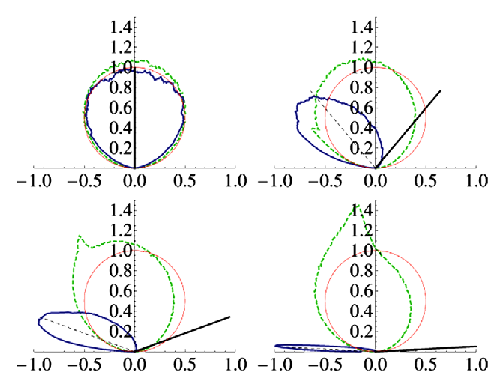
\includegraphics[width=6cm]{images/part1/2.eps}
    % Angular distribution of sputtered atoms (dashed) and reflected ions (solid) compared to a cosine distribution (circle) for incidence angles of 0°, 40°, 70° and 87°.
    \caption{Угловое распределение расплённыъ атомов(штрихпунктир) и отражённых ионов (сплошная) в сравнении с законом косинуса (круг) для углов падения \SIlist{0;40;70;87}{\degree}.}
    \label{fig:part1AngualarDistribution}
\end{figure}

\subsection{Вторичное распыление}

$IonShaper^{®}$ предпологает что переосаждённые атомы не распыляются и что отражённые ионы распыляются с таким же выходом как и падающие ионы. Чтобы посчитать достоверность этого предположения мы подсчитали средний выход распыления распылённых и обратно рассеянных ионов для нормального наклона ($Y_{ss}$ и $Y_{sb}$ соответственно) беря во внимание энергию распростронения распылённых ионов/обратно рассеяных ионов определённых симуляцией бинарных столкновений. Зависимость энергии нормально падающих распылённых ионов определенно с помощью аналитичной формулы. Т.к. в случае $Y_{ss}$ мы заинтересованы только в грубой оценке, мы приближаем выход распылённых $Si$ атомов распылением $Ar$ ионов.
Рис. ~\ref{fig:part1Yield} показывает выход вторичного распыления $Y_{ss}$ и $Y_{sb}$. Для сильно наклонённыех наклон $Y_{sb}$ близок к распылённию падающих ионов
($Y_{s} = 1.47$),
но оно уменьшается значительно когда угол падения уменьшается (пример на 30\% в 80; угол боковой стенки на Рис. ~\ref{fig:part1TrenchShape} между 77 и 86). Для контраста, средний выход распыления $Y_{ss}$ распылённых атомов скорее меньше и наверное незначительен в большенстве случаев.


\begin{figure}[h]
    \centering
    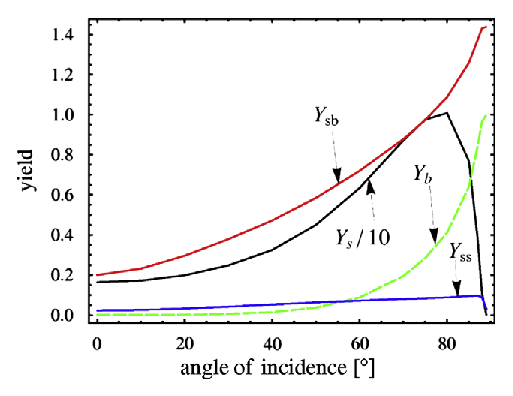
\includegraphics[width=6cm]{images/part1/3.eps}
    % Primary and secondary yields as a function of primary ion incidence angle as calculated by binary collision simulations
    \caption{Основной и вторичный выход как функция основного угла падения расчитанная симуляцией бинарных сталкновений }
    \label{fig:part1Yield}
\end{figure}

\subsection{Не локальные эффекты}

Чтобы исследовать нелокальные эффекты мы взяли контур на Рис. ~\ref{fig:part1TrenchShape} в 4.67с и посчитали основной поток распылённия в соответствии с разными моделями. Результаты полученные с локальной моделью показанны штрих-пунктирной линией на Рис. ~\ref{fig:part1Flux}, а результаты бинарного столкновения показанны сплошной линией. Можно заметить несколько удивительных отличий. Между 20нм и 50нм по абсциссе локальные результаты переоценивают поток. В первом случае это потому что луч ограничен \textgreater 20нм и вклад каскад отскоков столкновений ионов \textless 20нм пропущенно в результатах бинарного столкновия когда по иронии взято во внимание в локальной модели. В 50нм есть входящий поток \textgreater 50нм, но точки падений глубже чем если контур был бы расширен \textgreater 50нм с наклоном в \textless 50нм. Поэтому сложнее порождать отскоки от ионов в \textgreater 50нм чтобы вернуться к поверхности в \textless 50нм. Это отраженно в результатах бинарных столкновений но только в локальной модели. В 30нм видно два четких пика в локальной модели (положительный пик). Эти изминения в наклоне настолько стремительны что они не отраженны в результатах бинарных столкновений из-за эффекта размытия конечного размера каскадов отскоков.


\begin{figure}[h]
    \centering
    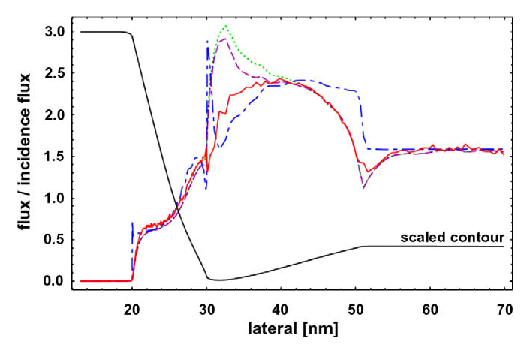
\includegraphics[width=6cm]{images/part1/4.eps}
    % Primary sputtering flux
    \caption{Основной поток распыления}
    \label{fig:part1Flux}
\end{figure}


Штриховая линия соответствует $IonShaper^{®}$ результатам полученным с табличной моделью отскоков описанных вместе с осаждённой моделью. Так же можно заметить что они совпадают с результатами бинарных столкновений в большей части случаев. Пик не представленный в результате бинарных столкновений может быть замечен только на дне микроямы (\textgreater 30нм). Это из-за того что путь от точки падения ион к точке назначения частично блокирован выгнутой поверхностю. Улучшенная модель описанная в конце секции 2.1 уменьшает этот пик, хотя некоторые отклонения от результатов бинарных столкновений остаются.

Наконец, Рис. ~\ref{fig:part1Deposition} показывает $IonShaper^{®}$ результаты вынужденного ионно-лучевого результата осаждения в 25нм границей 10К эВ $Ar$ лучём. Штриховая линия соответствует локальной модели когда сплошная линия представляет не локальную модель включая изменения отсков. Так же нужно заметить что конечные размеры каскада отскоков значительно увеличивают ширину осаждённгого столба. Этот эффект в основном выражен поскольку сравнительно низкая плотность отскоков вызывает значительный рост материала в ионно-лучевом осаждении.

\begin{figure}[h]
    \centering
    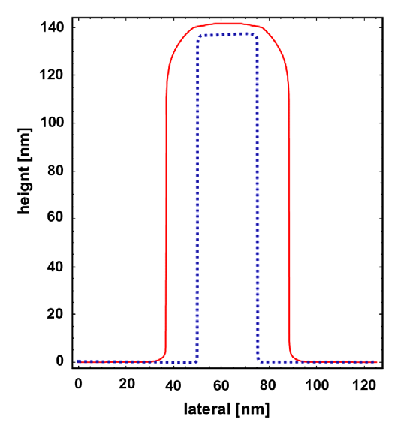
\includegraphics[width=6cm]{images/part1/5.eps}
    % Deposition of a pillar using a local model (dotted line) and a model considering the recoil range (solid line).
    \caption{Осаждение столба использующее локальную модель (точечная линия) и модель с отскоками (сплошная)}
    \label{fig:part1Deposition}
\end{figure}

\section{Выводы}
Наша оценка модели использованна для топографической симуляции ионой-лучевых процессов для 10К эВ $Ar$ ионов и $Si$ целей позволяет нам заключить следующее:

\begin{enumerate}
  \item Закон косинуса это только грубая аппроксимация углового распределения распылённых атомов. В особенности, распыление глубоких ям требует точного описания распределения на больщих обратных углах. Так же, зеркальное отражение это только грубая апроксимация для отражённых ионов. В обоих случаях реализация таблиц в топографическом симуляторе должна быть достачно хорошей.
  \item Как было показынно на Рис. ~\ref{fig:part1TrenchShape} распыление отражённых ионов может быть важным эффектом. Распыление распылённых частиц похоже несущественно из-за не значительного средней энергии распылённых атомов.
  \item Локальная модель распыления реализованная во всех топографических симуляторах на сегодня оказываеться достаточно неточна. Была предложенна модель основаная на пространственном распределении атомов на плоской поверхности и ожидается что она улучшает результаты на структурах малого размера. Нелокальная модель даже более важна для ионно-лучевого осаждения.
\end{enumerate}

Мы планируем расширить эту работу на другие энергии и типы ионов, изучать влияние предложенных моделей на форму поверхностей.

\section{Благодарности}

Эта работа было частично поддерженна Европейской коммисией путём финансирования проекта CHARPAN и Австрийским агенством продвижения, Австрийской нано инновационной программой, проектом NILaustria.


%
% Another article
%

\newcommand{\fib}{(\textbf{\uppercase{fib}})}

\newcommand{\dd}{\textbf{\uppercase{2d}}}
\newcommand{\dt}{\textbf{\uppercase{3d}}}

\newcommand{\desccharpan}{\textbf{\uppercase{charpan}} (\textbf{Char}ged \textbf{Pa}rticle \textbf{N}anotech)}
\newcommand{\charpan}{\textbf{\uppercase{char\-pan}}}

\newcommand{\ion}{$IonShaper^{®}$}


\part{Симуляция прямого ионного формирования \dt{} нанопечатей}


\section{Введение}

Проекция ионного луча было предложено многими группами как обнодёживающий вариант улучшить эфективность в производстве с использованием распыления по отношению к обычным технологиям фокусированного луча \fib{}. Идея такова: использовать трафарет или програмируемую щелевую подложку, предлагающую \dd{} структурированный ионный профиль для ионного фрезерования, травления, и осаждения. Главное приемущество использовать \dd{} структурированных лучей вместо фокусированных лучей \fib{} для определённых приложений в том что что продуктивность может быть улучшенна на более чем два порядка (как для всего потока так идля точечного отношения). Это в особенности справедливо для приложений где предварительный газ используеться для химических улучшений процесса (травления и осаждения), хотя плотность потока у ширины луча достатчно мала чтобы избежать пространственного истощения газа. Более того, \dd{} структурированный луч позволяет очень точно контролировать уровни ионого влияния. Последний играет роль в формировании \dt{} поверхностей с требованиям нанометровой точности формы или для высоко чувствительных к облучению материалов, для примера, органичекие тонко плёночные структуры. Интегрированный европейский проект \desccharpan{} был запущен чтобы использовать эти приемущества и с целью эксплуатировать ионно-лучевой средства для формирования образцов для наномаштабного производства.

\section{Модель симуляции}

Модель размывания, использованная для симуляции в программе \ion{}, подражает натуральному процессу описанному вектором скорости нормальным к поверхности и формой поверхностью с полной производной. Однако, последнее условие в основном не выполняеться в базовой размытой симуляции. В реальности, существует предел для максимальной кривизны которая может быть развита из-за эффектов рельных размеров таких как пространственная диффузия или каскады столкновений пространственно разделяют падающих ионов и расплённых атомов. Размытые симуляции которые не включают естественное сглаживание или чья длина дискретизации больше чем упомянутый атомистичный эффект должны справляться c особенностями производной форсы поверхности. Иммено поэтому в модели размывания \ion{} реализованна специальная обработка поверхностей границ: простейшие модели размытия описывают эволюцию поверхности либо как паралельное движение достаточно коротких участков либо движение индивидуальных точек перпендикулярно основной поверхности.

\begin{figure}[h]
    \centering
    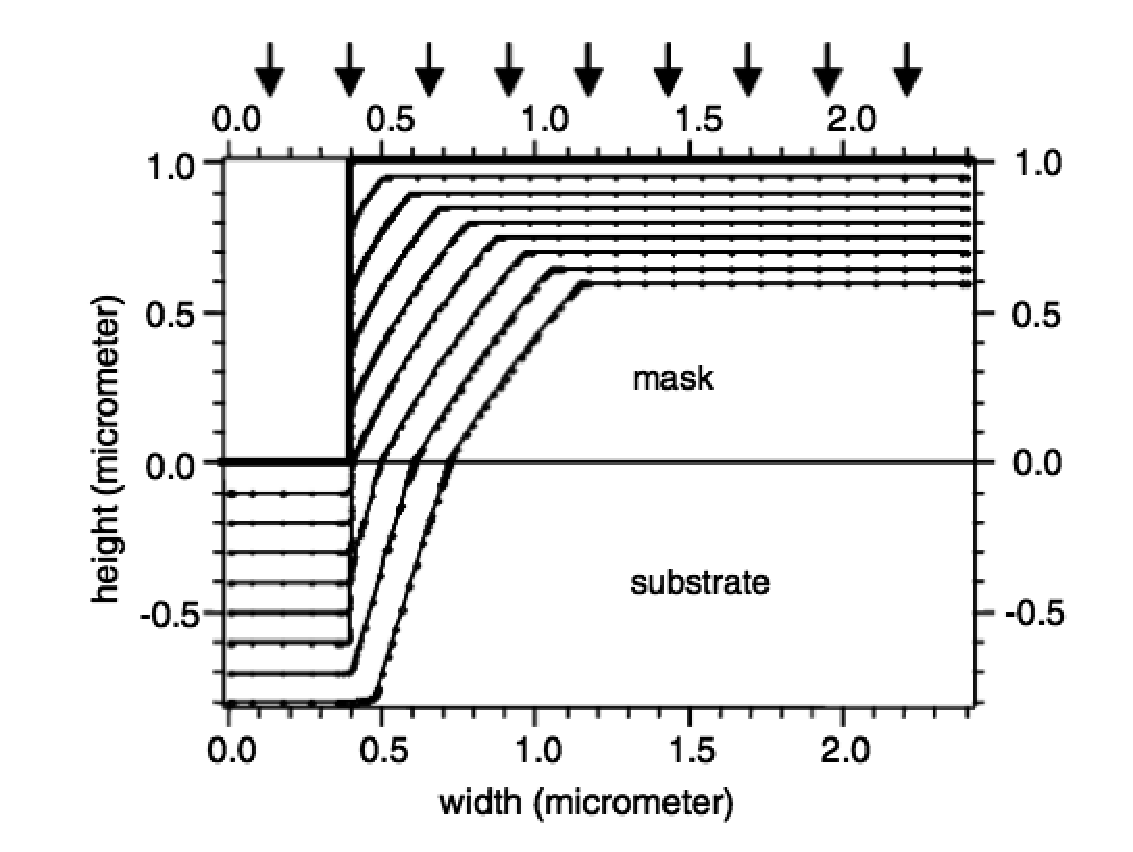
\includegraphics[width=6cm]{images/part2/1.eps}
    \caption{\ion симуляция}
    \label{fig:part2IonShaper}
\end{figure}

\newpage
Наша модель сочетает оба метода чтобы гарантировать точную симуляцию "чётких" граней где наклон поверхности плохо определён. Первое, макимальных угол между смежными сегментами ограничен меньше \ang{20} - \ang{45}. Второе, в дополнение к средниму наклону два индивидуальных наклона сегментов с обоих сторон поверхности указанных в вопросе также использовались для того чтобы определить наибыстрейщую прямую тракторию движения и поверхнсть точек движется соотвественно но всё равно перпендекулярно к среднему наклону. Включая эти корректировки, \ion{} главная модель эрозии способна воспроизвести результаты математически более изощрённых подходов основаных на общей теории теории Гюгенса, которая может иметь дело с бесконечно остроыми краями. Приемущеста нашей модели эрозии - это очень простая реализация высокоуровневых эффектов таких как переосаждение и второичная эрозия от отражённых ионов.

\begin{figure}[h]
    \centering
    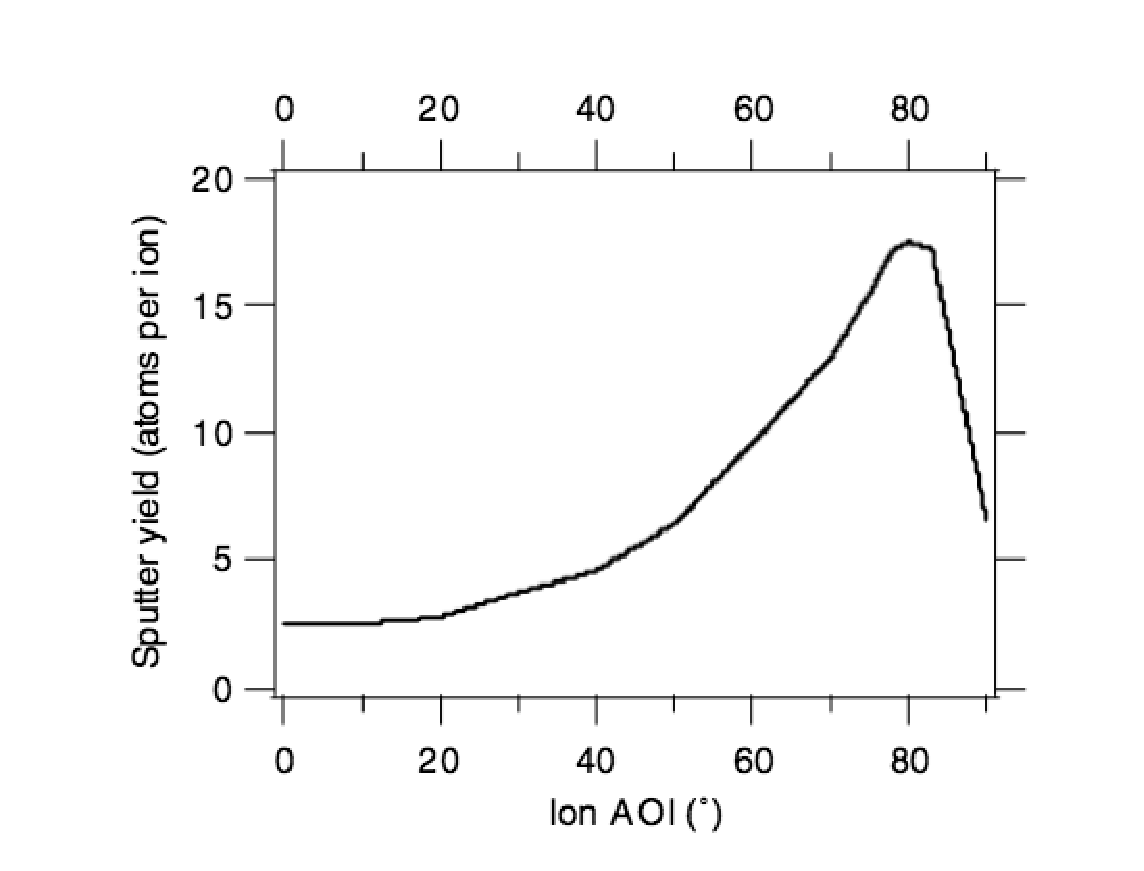
\includegraphics[width=6cm]{images/part2/2.eps}
    \caption{Зависимость распылённого выхода от угла падения ионов основанное на эксперементальных данных}
    \label{fig:part2SputterYield}
\end{figure}

Атомические эффекты неявно включенны изменением различных параметров симуляции в атомистичной симуляции Монте-Карло,для примера, угол зависимый от ионого распыления. Критичные и эксперементально доступные параметры как угловая зависимость расплёного выхода взяты напряму из эксперемента (Рис. ~\ref{fig:part2SputterYield}).

(Рис. ~\ref{fig:part2IonShaper}) показывает \ion{} симуляцию приложенную к идеально бинарной, для примера, маск-подложка где распылённый выход на маск-уровне является половиной жтой подложки. Читателель поощряеться сравнить эти результаты с "точными" численненной симуляцией использующей обобщенную теорию Гюгенса данную в ссылке 5, откуда очивидна согласовонность теории с симуляцией. Также нужно заметить сосредоточение сегментов около углов и пересечение двух слоёв маски и (подложки) из-за динамической сетки реализованной в \ion{}.

\newpage

\begin{figure}[h]
    \centering
    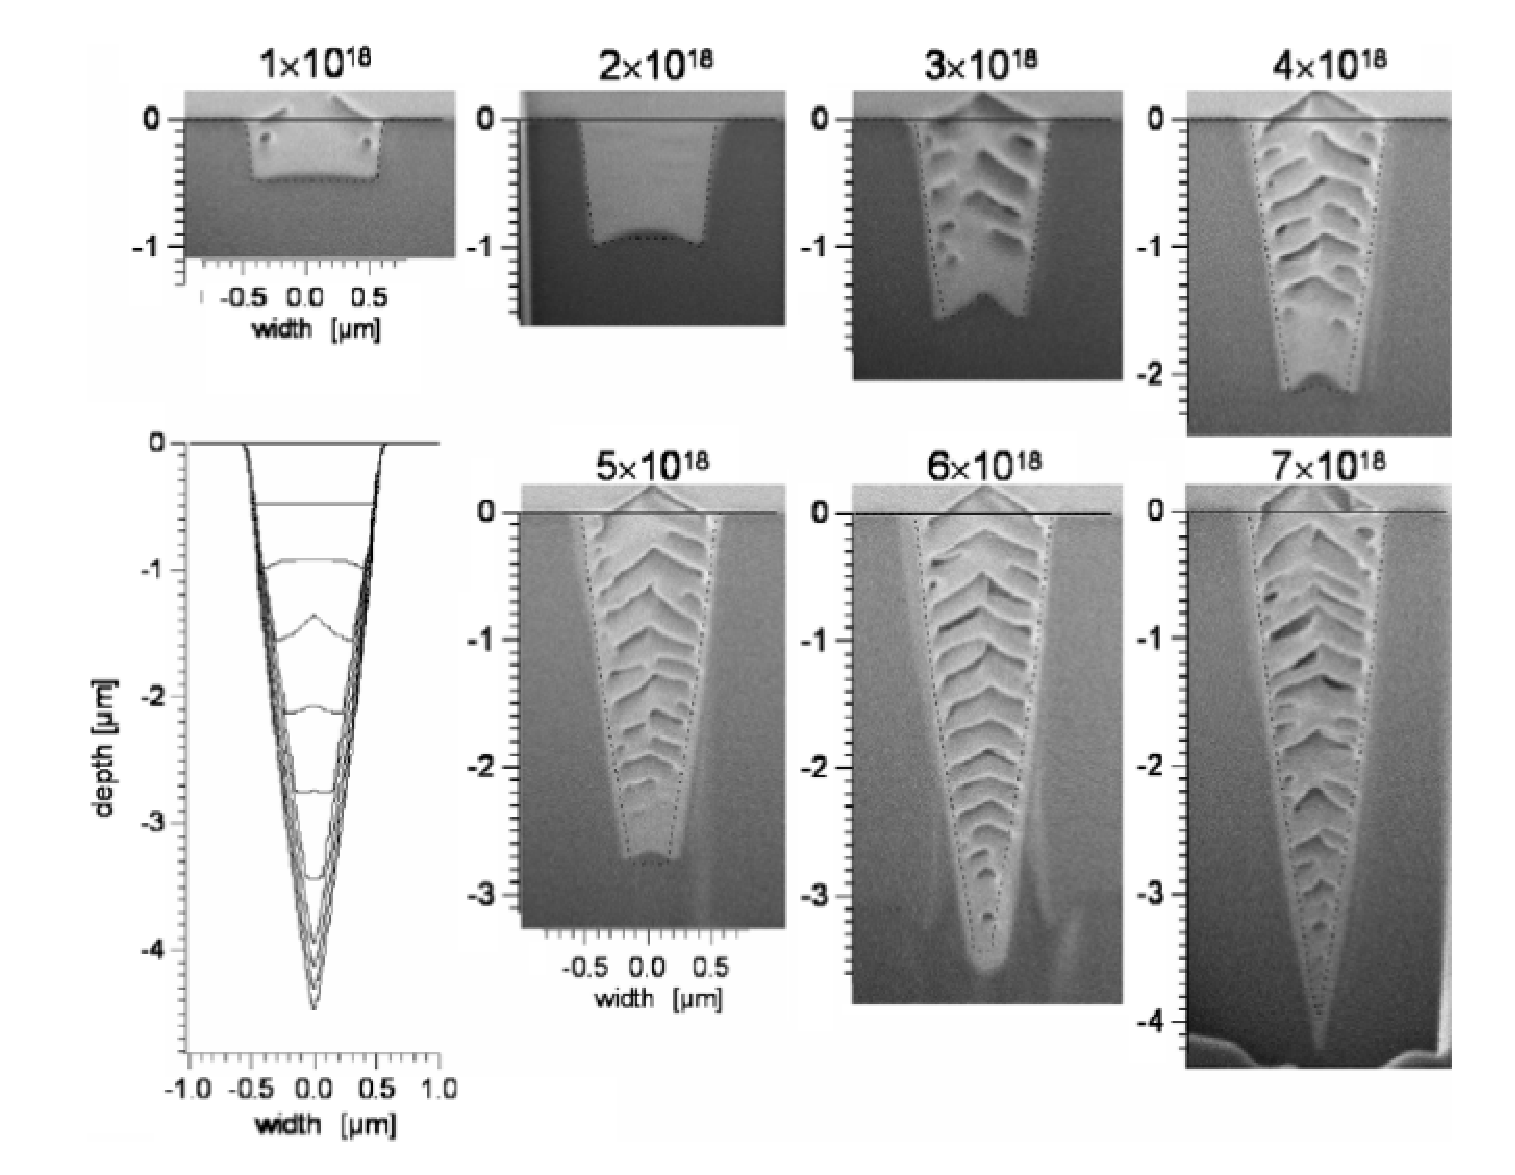
\includegraphics[width=15cm]{images/part2/3.eps}
    % \caption{Зависимость распылённого выхода от угла падения ионов основанное на эксперементальных данных}
    \caption{Профили ямы}
    \label{fig:part2Many}
\end{figure}

\section{Решения}


\ion{} результаты также сравними с эксперементальными результатами полученными из фокусированных ионнно-лучевых процессах распыления. Для этих целей, $Si$ подложка была облученна 30 keV $Ga$ ионами. Фокусированный ионный луч имел полную ширину 70 нм и был направлен на образец через прямоугльный фильтр с полосой пропускания 12.5 нм. На протяжении процесса этот растр повторяли много раз чтобы достич локальный ионный поток \SIrange[per-mode=fraction]{1e18}{7e18}{\siion\per\square\centi\meter}. Это показанно в расплыённой яме шириной 1 мкм нескольно микрометров глубиной и примерно 10 мкм длиной. После распыления они были наполнены металлом в$FIB$ вынужденном процессе напыления. Чтобы проверить форму ямы, $FIB$ меж-секции были сделанны перпендикулярно к ямам. На (Рис. ~\ref{fig:part2Many}), показанна последовательность вторичных электронных картинок меж-секций ямы. После накопления ионного потока в \SI[per-mode=fraction]{1e18}{\siion\per\square\centi\meter} яма около 0.5 мкм глубиной с почти плоским дном. С увеличением потока наблюдается две характерестичные черты: яма становиться более узкой а дно W-образным. Первый эффект из-за переосаждения распылённых атомов подложки. С увеличением отношения сторон ямы вероятность прилипнуть распылённым атомам к противоложенной стенки так же возрастает. W-образная форма вызвана увелиенным распылением в углах на дне из-за ионного рассяния  не вертикальной стороны. W-образная форма наиболее выраженна когда яма достигает соотношение сторон 1.5-2.0. После этого характерная форма дна сглаживается из-за налажения интенсивностей рассеяных ионов с обоих стенок. Дно становится ровным с обоих стенок и процесс заканчивается с V-образной формой ямы с соотношение сторон равным 4.



При сравнении с эксперементальными данными, симуляция воспроизводит все основные особенности описанне выше как качественно так и количественно. Симулированные кривые на Рис. ~\ref{fig:part2Many} не были полученны путём подгонки, они результат подсчёта с одним набором параметров симуляции. Есть только одно не большое расхождение между симуляцией и реальным контуром осмотримом на высоком потоке \SI[per-mode=fraction]{6.5e18}{\siion\per\square\centi\meter}. В таком режиме симуляция недооценивает рыспылённую глубину. Мы предпологаем что этот эффект возникает от двойного или много разового рассеения от стенок которое не включенно в \ion{} модель симуляции, которое может вызывать усиление эффекта ионной фокусировки.

\begin{figure}[h]
    \centering
    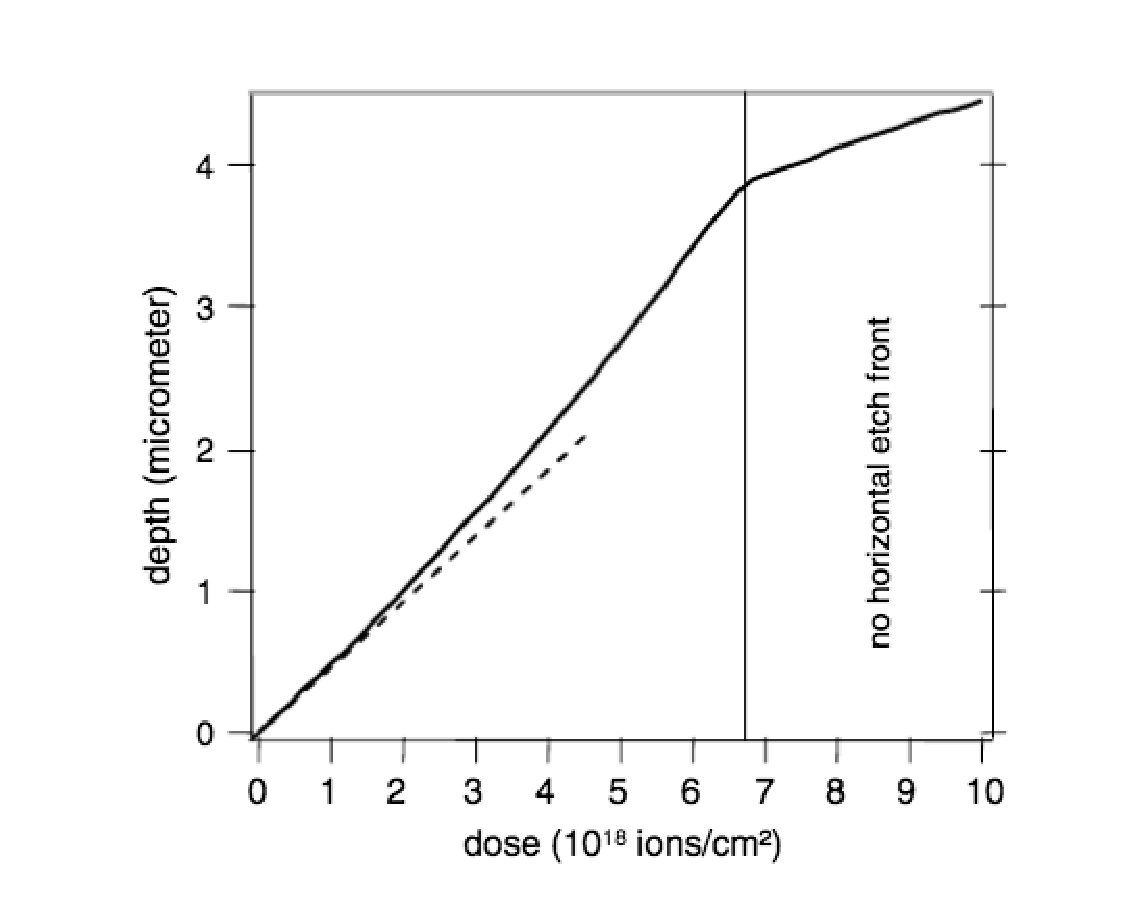
\includegraphics[width=6cm]{images/part2/4.eps}
    \caption{Зависимость глубины от потока ионов}
    \label{fig:part2Depth}
\end{figure}


Начальное ускорение следующее за замедлением скорости эрозии на больших соотношения сторон являеться ешё одним интересным свойством, показанно на Рис. ~\ref{fig:part2Depth}. Когда ямя становится глубже переосаждение материалла расплылённого в глабоких частях ямы приводит к более и более узкой яме. В начале, фокусировка ионов отраженных накланённых стенок ямы усиливает частоту травления. Иногда, однако, близко к середине ямы фокус исчезает, что вызывает внезапное замедление процесса эрозии. Переосаждение и тем самым сжатие ямы может быть строго предотвращено путём использования травления в атмосфере газа, который препятствует переосаждению в следствии химических реакций. Это приводит к формированию прямоугольной ямы с высоким соотношением сторон.

В дополнение к распылённой симуляции, \ion{} может буть использован для симуляции вынужденного ионного осаждения где энергия подающих ионов превращает абсорбированный предварительный газ на подложке в неизменный осадок похожий на процесс химического парового осаждения ($CVD$). Однако, использование упорядоченного ионного луча приводит к очень высокой пространственному разрещению процесса осаждения. Недавно было продемонстрирован автономный рост около 100 нм проводов. [6]. Рис. ~\ref{fig:part2Growth} показывает симуляцию роста вертикальных нанопроводом для трех различных пиковых потоков плотности ионов использующих ультра изкий ионный луч меньше чем 10 нм шириной (12 нм  $FWYM$, с 1.0.1, и 0.01 pA током соответственно).

\begin{figure}[h]
    \centering
    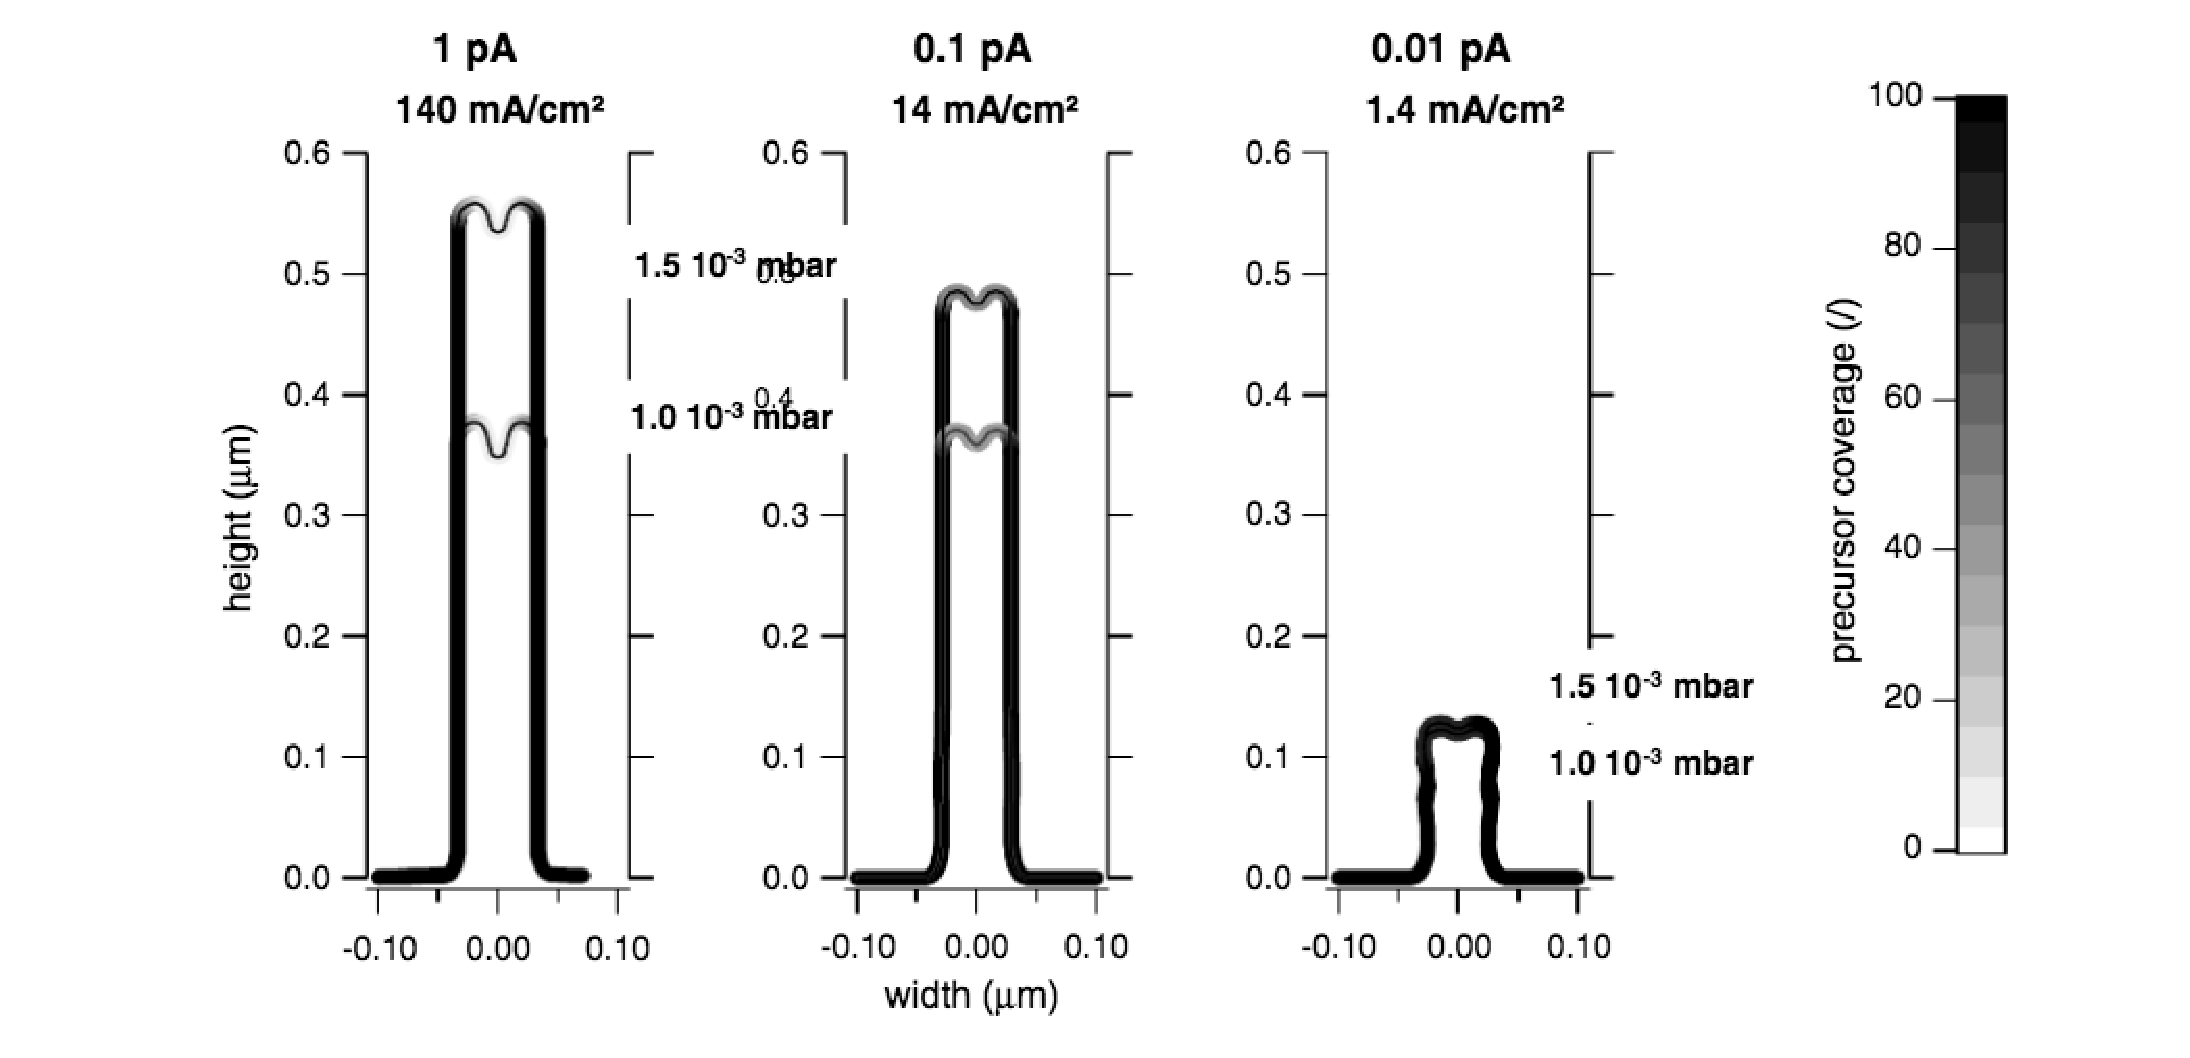
\includegraphics[width=15cm]{images/part2/5.eps}
    \caption{Симуляция роста нановолокна}
    \label{fig:part2Growth}
\end{figure}

\newpage

Этот пример показывает взаимодействие предворительного растворения, осаждения, и распыления. Разделение предварительного газа предпологается вызвана вторичными электронами. Мы берём это во внимание предполагая ширину ионного-лучевого действия радиусом 25 нм и выходом осаждения 10. Соответственно ионый луч гораздо уже чем нанопровод. Диаграммы показывают осаждение . Диаграммы показывают осаждение . Диаграммы показывают осаждение . Диаграммы показывают осаждение . Диаграммы показывают осаждение . Диаграммы показывают осаждение . Диаграммы показывают вынужденное осаждение от ионных лучей с высокими ионными токоми в основном используемых для $FIB$ процессов.Заметна строгая зависимость скорости роста от давления предварительного газа. В этих условиях рост ограничен растворением предварительного газа и тем фактом что большая часть потока ионов не имеет ни какого эффекта кроме как распыления изкой ямы ограниченного размера (Рис. ~\ref{fig:part2Many}) в центре нановолокна.

Однако, для технических приложений органиченных рост ионного тока может быть даже выгоден потому что очень сложно контролировать локально поглощение предварительного газа. Ещё одна диаграмма показывает текущую ограниченную натуру плотности процесса роста вынужденого сравнительно низкой плотностью потока используемой в средствах разработанных в \charpan{}. В этом режиме потока, предварительный газ, с его давление, почти что не иммет эффекта на частоту роста потому что сокрашение газа не наблюдается.

Использование низкой плотности тока, для примера, плотность потока показанное в \charpan{} может обеспечить около 20 кратно быстрый рост нановолокон в сравнении с $FIB$ процессом. Это справедливо для больших площадей осаждения. Беря во внимание возросший общий допустимый ток с ионной проджекцией ( более чем 2 раза) потенциал производста а наномасштабе более чем очивиден.

\section{Выводы}

Производсто \dt{} поверхностных структур путём прямой ионной-лучевой обработки - это интересная возможность для различных применений включая формирование наноштамнов. Контролируемое \dt{} производство требует настройку сумулятора на связанный процесс повторения.  В этой статье, симуляционная программа \ion{} предлагает превосходный контроль процесса для ионно-лучево распыления, вынужденного ионного травления, и осаждения.

\end{document}
